\chapter{Trabalhos Relacionados}
\label{chap2}

\section{Soluções existentes de interação com o banco de dados}

\subsection{Neo4j Browser}
A principal ferramenta utilizada para interagir com os dados no banco de dados Neo4j é o Neo4j Browser. Software proprietário da empres. Que contém uma linha de comando que permite todas as operações de CRUD, através de execução de cyphers.


\begin{figure}[H]
    \centering
    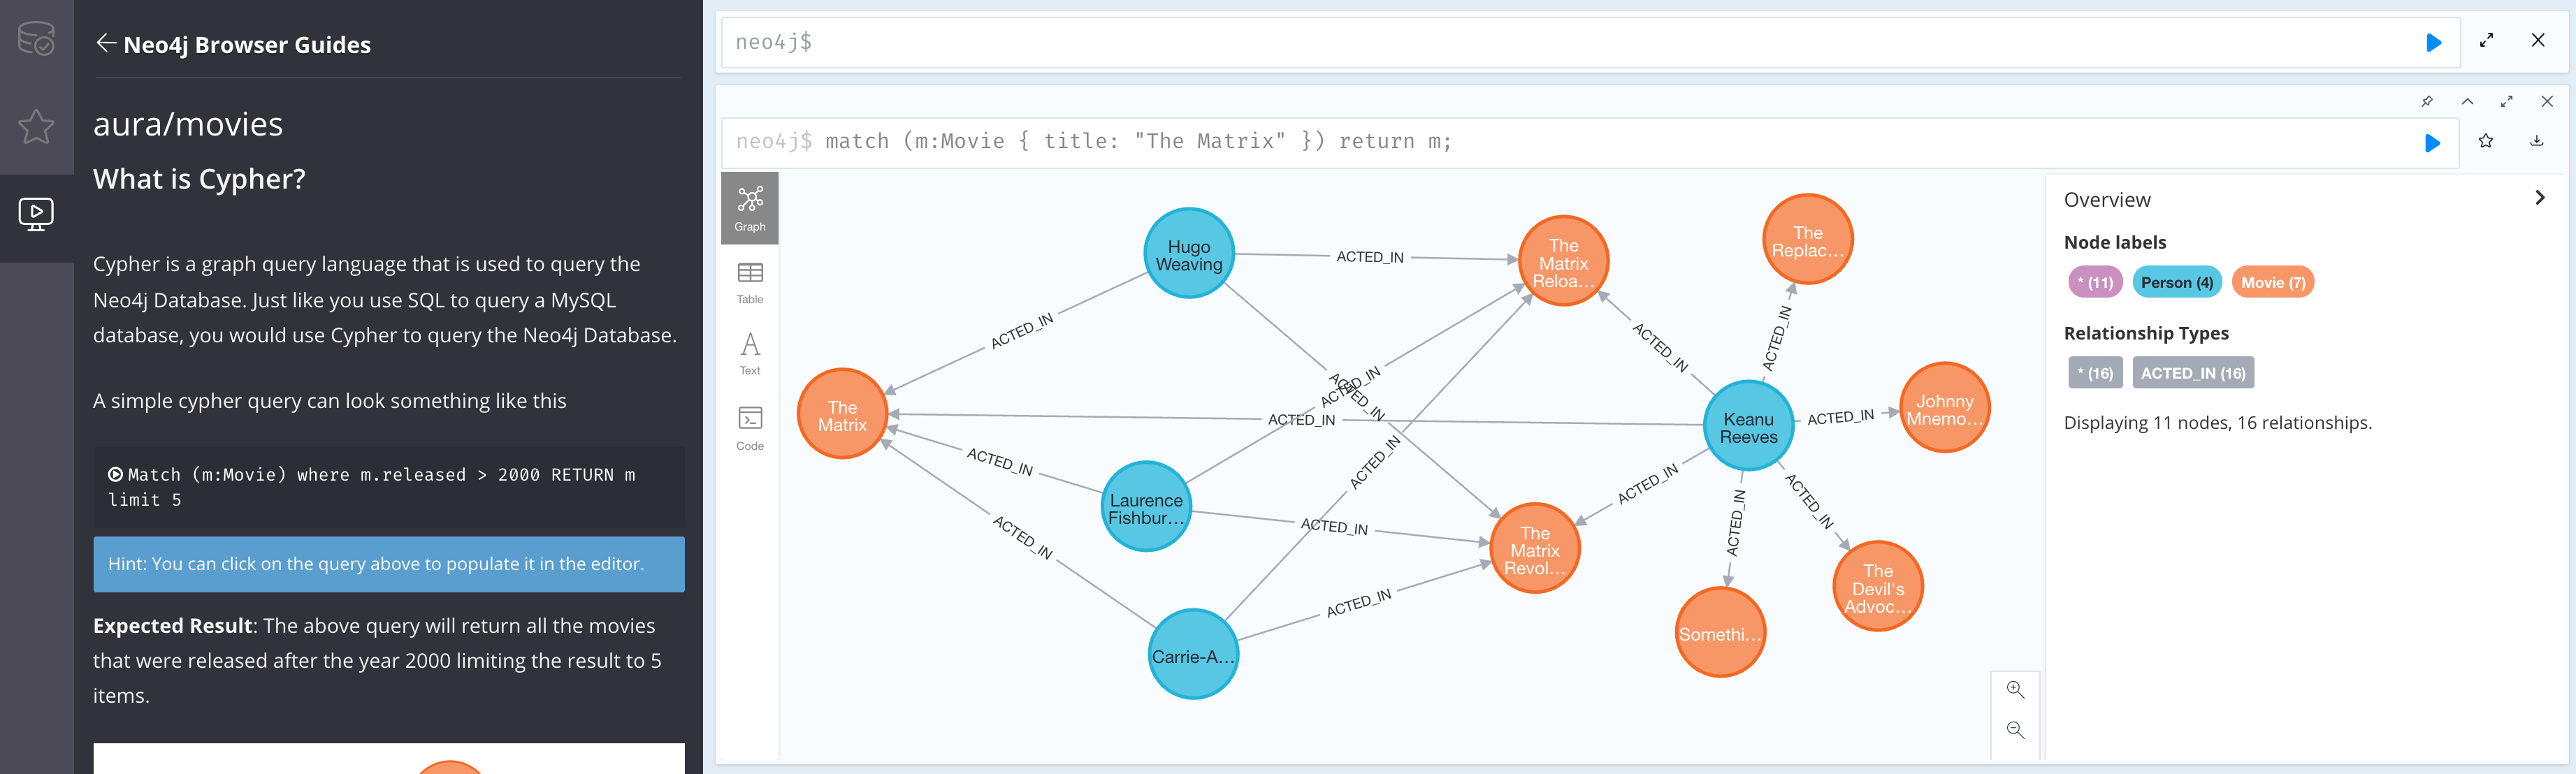
\includegraphics[width=1.0\linewidth]{Imagens/chap02/neo4j-browser-oneshot.png}
    \caption{htps://dist.neo4j.com/wp-content/uploads/neo4j-browser-oneshot.png.}c
    \label{fig:profile-exemple}
\end{figure}

É muito poderoso, especialmente dada o vasto ferramentário disponibilizado pela bilbioteca APOC (Awesome Procedures On Cypher), porém isso pode ser entendido como ônus para alguns casos de uso. No momento que uma quantidade de usuários maior precisa interagir de maneira administradora nos dados, e que a quantidade de nós é significativa, uma desatenção pode causar uma requisição pesada demais para o sistema gerenciador, causando problemas de instabilidade para todos os usuários que interagem com o grafo.

Outrossim, permite realizar amplas alterações nos dados do grafo, de difícil reversão.

\subsection{Neo4j Bloom}

Neo4j Bloom é uma ferramenta de visualização e interação com grafos em bancos de dados Neo4j, sem necessitar de Cyphers. Ele surge como uma alternativa ao Browser. No Bloom, podemos selecionar padrões de nós e conexões no grafo, e visualizar os dados que o seguem, com a capacidade de editar as conexões e propriedades dos nós.

\begin{figure}
    \centering
    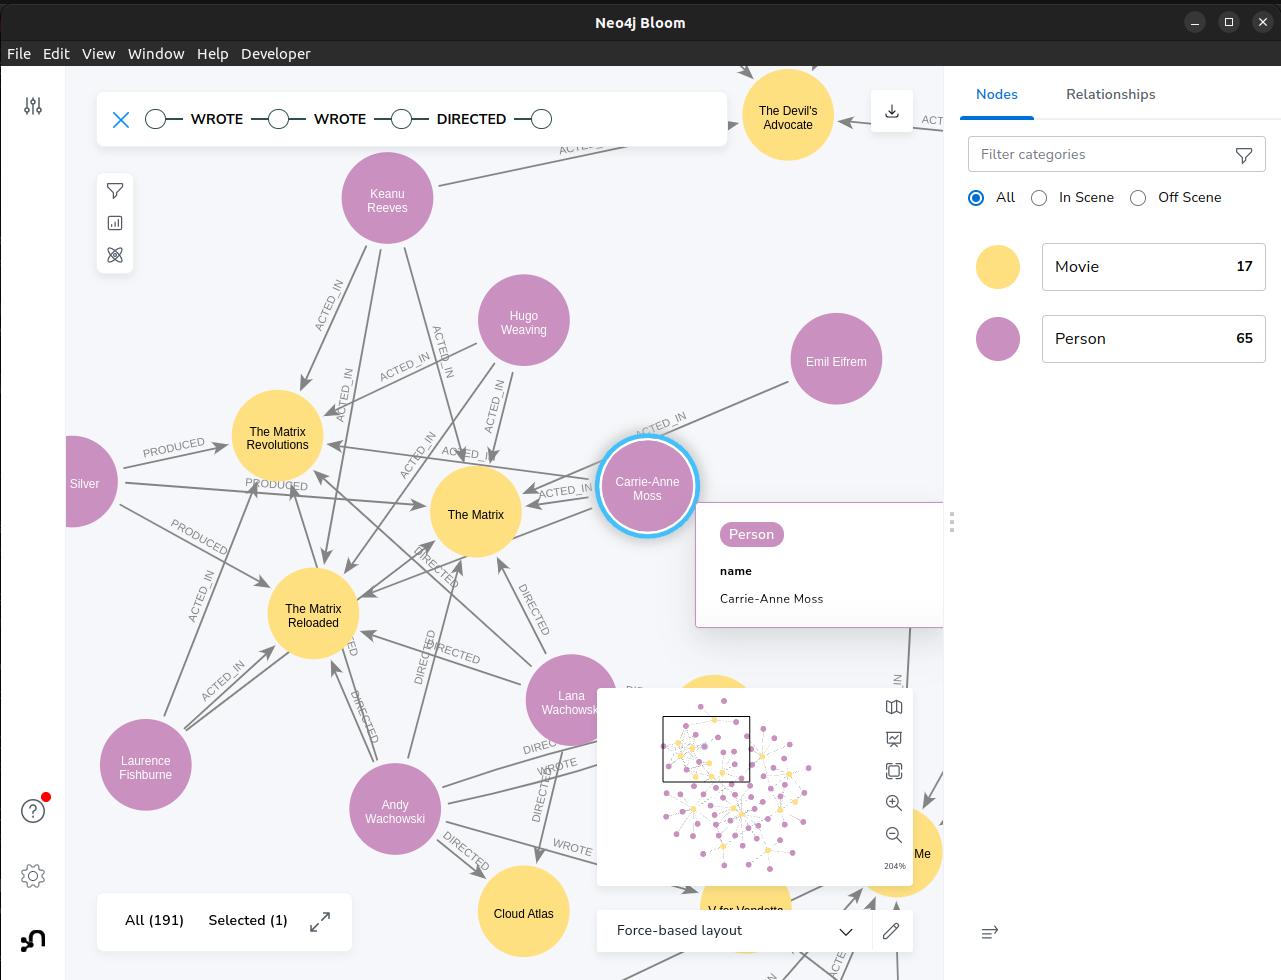
\includegraphics[width=0.8\linewidth]{Imagens/chap02/neo4j-bloom.png}
    \caption{Interface do Neo4j Bloom visualizando uma base de dados de filmes e atores.}
    \label{fig:neo4j-bloom}
\end{figure}

O Neo4j Bloom acrescenta uma camada de segurança comparado ao Neo4j Browser, dificultando modificações extensas ou consultas demasiadamente intensiva em recursos para o banco de dados. Ele, porém, ainda obriga o conhecimento do usuário sobre o schema do banco de dados e os padrões existentes e relevantes encontrados nele.

Além disso, permite interação diretamente com o Neo4j, sem passar pelas definições de \textit{tipos} no servidor. Isso significa que é possível editar qualquer nó e relacionamento acrescentando qualquer propriedade, fugindo dos padrões de cada \textit{tipo}. Tal liberdade dificulta o gerenciamento do dados, e acrescenta possibilidade de erros críticos que quebrem funcionalidades chave das plataformas.

\subsection{Neo4j Developer Graph Apps Gallery}

A Neo4j Inc. permite e estimula a criação de aplicativos por terceiros para gerenciamento, análise e visualização de dados que se comunicam com seus bancos de dados. Alguns desses aplicativos são disponibilizados em uma Galeria curada pela própria Neo4j e disponibilizada para integração com seu banco através do software Neo4j Desktop. 

Dentro das ferramentas disponíveis, algumas permitem a interação e edição direta com o banco de dados, podemos citar o Neo4j Commander 3. Porém sempre esperando do usuário um conhecimento sobre o schema e seus padrões em grafos, com interfaces elaboradas e curva de apredizagem extensas.

Na falta de uma ferramenta que permite o gerenciamento de dados de maneira intuitiva e segura para usuários não-técnicos, a desenvolvemos internamente.
